\chapter{The Secure Layer \label{chap:ssl}}

Transport Layer Security, formerly known as SSL (Secure Socket Layer), aims
to bring some security features over a communication channel, specifically
providing \strong{integrity} and \strong{confidentiality} of the message,
\strong{authenticity} of the server and optionally the client.
%% fuck osi layers: there is no code explicitly structuring the internet in 7
%% layers.
Many ancient application protocols wrapped themselves to be over TLS/SSL, with
the only difference of the ``s'' appended to the protocol name (such as HTTPs,
IMAPs). It is nowadays widely adopted all over the world, becoming the de-facto
standard for end-to-end  encryption.

\paragraph{Certification Authorities} are authorities to whom it is granted the
power to \emph{authenticate} the peer. Pragmatically, they are public keys
pre-installed on your computer that decide who and who not to trust by employing
a digital signature.
In order to overcome the proliferation of keys to be distributed, and satisfy the
use-case of a mindless user willing to accomplish a secure transaction on the
internet, the following, hierarchical trust model proliferated (~\cite{rfc4158},
Fig.2)\footnote{
  The image is merely esemplificative, there is no boundary to the structure of
  the tree.}:
\\
\\
%% E` BELLISSIMO QUESTO COSO
\begin{center}
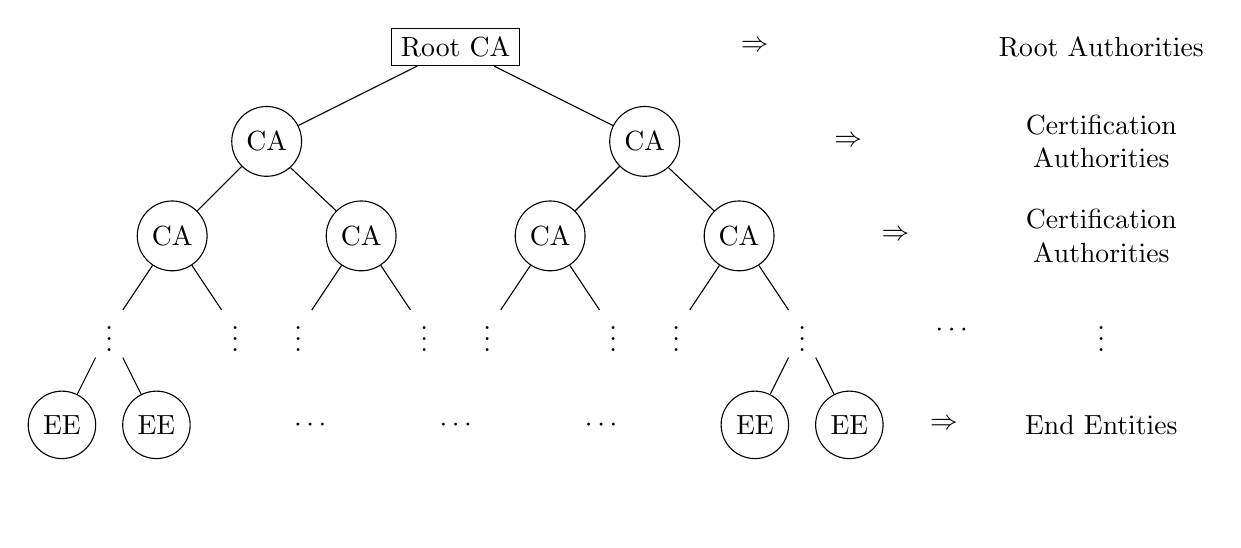
\begin{tikzpicture}[
  scale=0.8,
  align=center,
  level/.style={sibling distance=60mm/#1}]
\node [draw] (z){Root CA}
  child {node [circle,draw] (a) {CA}
    child {node [circle,draw] (b) {CA}
      child {node {$\vdots$}
        child {node [circle,draw] (d) {EE}}
        child {node [circle,draw] (e) {EE}}
      }
      child {node {$\vdots$}}
    }
    child {node [circle,draw] (g) {CA}
      child {node {$\vdots$}}
      child {node {$\vdots$}}
    }
  }
  child {node [circle,draw] (j) {CA}
    child {node [circle,draw] (k) {CA}
      child {node {$\vdots$}}
      child {node {$\vdots$}}
    }
  child {node [circle,draw] (l) {CA}
    child {node {$\vdots$}}
    child {node (c) {$\vdots$}
      child {node [circle,draw] (o) {EE}}
      child {node [circle,draw] (p) {EE}
        child [grow=right] {node (q) {$\Rightarrow$} edge from parent[draw=none]
          child [grow=right, xshift=1cm] {node (q) {End Entities} edge from
            parent[draw=none]
            child [grow=up] {node (r) {$\vdots$} edge from parent[draw=none]
              child [grow=up] {node (s)
                {Certification\\ Authorities} edge from parent[draw=none]
                child [grow=up] {node (t)
                  {Certification\\ Authorities} edge from parent[draw=none]
                  child [grow=up] {node (u) {Root Authorities} edge from
                    parent[draw=none]}
                }
              }
            }
          }
        }
      }
    }
  }
};
\path (o) -- (e) node (x) [midway] {$\cdots$}
  child [grow=down] {
    %%node [draw] (y) {End User}
    edge from parent[draw=none]
  };
\path (u) -- (z) node [midway] {$\Rightarrow$};
\path (s) -- (l) node [midway] {$\Rightarrow$};
\path (j) -- (t) node [midway] {$\Rightarrow$};
%% \path (y) -- (x) node [midway] {$\Downarrow$};
\path (e) -- (x) node [midway] {$\cdots$};
\path (o) -- (x) node [midway] {$\cdots$};
\path (r) -- (c) node [midway] {$\cdots$};
\end{tikzpicture}
\end{center}
\vfill

There are two types of authorities: root CAs and intermediate CAs. Root
Authorities are the only nodes ultimately considered trustoworthy by the end
user. Their private key is used to sign digital certificates, either to
Certificate Authorities, to which is delegated the power of authenticating
others, or End Entities, holders of a private key and their corresponding
certificate whose identity has been verified.

Upon connecting, the client will check to see if the certificate presented was issued
by a CA present in the trust store (root CA); otherwise it will check to see if
it has been issued by a trusted CA, and so on until either a trusted CA is
found or no trusted authority is found. In the latter case, the connection is aborted.

\paragraph{The protocol} is actually a collection of many sub-protocols:
\begin{itemize}
  \setlength{\itemsep}{1pt}
  \setlength{\parskip}{0pt}
  \setlength{\parsep}{0pt}
\item \strong{\emph{handshake}} protocol, a messaging protocol that allows to
  \emph{authenticate} the peers, and eventually restore a past encrypted
  session.
\item \strong{\emph{record}} protocol, permitting the encapsulation of higher level protocols,
  like HTTP and even the next two sub-protocols. It is the fulcrum for all data
  transfer.
\item \strong{alert} protocol, which steps-in at any time from handshake to closure of the
  session in order to signal a fatal error. The connection will be closed
  immediately after sending an alert record.
\item \strong{changespec} protocol, to negotiate with and notify  the receiver that
  subsequent records will be protected under the just negotiated keys and
  \texttt{Cipher Spec}.
\end{itemize}
We will now proceed with a brief synopsis of the first two of these protocols,
due to their relevant role inside the connection, but will not proceed further,
as they were the only two we actually used in our research.


\section{The \texttt{handshake} protocol}
As mentioned above, the handshake occurs whenever a machine attempts to start
a TLS connection. If there is no session identifier, a new one is being built
up; otherwise the client will include the session-id in the initial
communication and the server will eventually skip the key agreement phase since
%% XXX. check the use of verb happened
it has happened recently\footnote{``recently'' is not well-defined in
  the standard - it is suggested an upper limit of 24-hours lifetime, but the
  only actual constraint is that both client and server agree on it.}.\\
A new session identifier gets built as follows. Once a communication channel
over the transport layer has been established, the client sends a hello
message, to which the server must respond with a server hello, or else a fatal error
will occurr. The above hello messages agree the two parties on the TLS protocol
version, compression and encryption methods, and  establish a session identifier
(\cite{rfc2246} \S 7.3).

Following the hello messages, the server will send its certificate,
if it is to be authenticated. If the client is happy with it, a RSA or
Diffie-Hellmann key exchange is initiated by the client to establish the
symmetric key to be used for the ensuing session.

\section{The \texttt{record} protocol}
Once the two parties share a common secret, called \emph{premaster secret},
they can generate a new key to be used for symmetric encryption of message, and
another for message authentication.

All TLS protocol messages move in records of up to 16K, containing 3
main components: MAC-data, data, and padding.
\begin{itemize}
\item {MAC-data} is no other than the Message Authentication Code over the
encrypted \emph{data} sent
(SSL performs the encrypt-then-mac mode of operation).
It provides \strong{authenticity} and \strong{integrity} of the message.
\item {Data} is the actual message, encrypted after an eventual compression.
\item The {Padding} section contains informations about the padding algorithm
adopted, and the padding size.
\end{itemize}
Failure to authenticate, decrypt will result in I/O error and a close of the
connection.

\section{What is inside a certificate \label{sec:ssl:x509}}
SSL certificates employed the X.509 PKI standard, which specifies, among other
things, the format for revocation lists, and certificate path validation
algorithms.
\\
\begin{center}
  \scalebox{0.7}{
    \begin{bytefield}[bitwidth=0.95em]{16}
      \begin{rightwordgroup}{Certificate}
        \wordbox{1}{Version} \\
        \wordbox{1}{Serial Number} \\
        \wordbox{1}{Algorithm ID} \\
        \wordbox{2}{Validity \\ \tiny{$\angular{\text{NotBefore, NotAfter}}$}} \\
        \wordbox{2}{Issuer \\ \tiny{eventually plus Issuer Unique Identifier}} \\
        \wordbox{2}{Subject \\ \tiny{eventually plus Subject Unique Identifier}} \\
        \wordbox{2}{Subject Public Key Information \\
          \tiny{$\angular{\text{PubKey algorithm, PubKey}}$}} \\
        \wordbox[lrt]{1}{Extensions} \\
        \skippedwords  \\
        \wordbox[lrb]{1}{}
      \end{rightwordgroup} \\
      \wordbox{1}{Certificate Signature Algorithm}  \\
      \wordbox{1}{Certificate Signature} \\
    \end{bytefield}
  }
\end{center}

It is a pretty old standard, defined in the eighties by the ITU.
Born before HTTP, it was initially thought \emph{in abstracto} to be
extremely flexible and general\footnote{
  \textit{``X.509 certificates can contain just anything''} ~\cite{SSLiverse}
}.
And precisely for this flexibility and its adaptation to the SSL/TLS protocol
without a very-well defined structure have been its major flaws: it is still
difficult to write good, reliable software parsing a X.509 certificate.

\section{Remarks among SSL/TLS versions}

The first, important difference to point out here is that SSLv2 is no more
considered secure. There are known attacks on the ciphers adopted (md5, for
example \cite{rfc6176}) as well as protocol flaws.
SSLv2 would allow a connection to be closed via a not-authenticated TCP segment
with the \texttt{FIN} flag set (\cite{rfc6176} \S 2). Padding informations are sent in
clear, and the payload is not compressed before encrypting, allowing a malicious
attacker traffic analysis capabilities \cite{sslpadding}. The ciphersuite is negotiated using
non-authenticated informations, allowing an attacker to influence the choice of
the \texttt{Cipher Spec} and weaken the security of the communication
\cite{rfc6176} \S 2.
Most of these vulnerabilities have been addressed by the later SSLv3, which
introduced compression and protection against truncation attacks.
Its standardized twin, TLS 1.0, only differs on the cipher suite and key
calculation requirements, strengthen in order to increase the security of the
channel \cite{rfc2246}.
Both SSLv3 and TLS 1.0 have been threatened in 2011 by an attack that could break
the same origin policy, known as BEAST. It is not dramatic, and almost any
browser now mitigates its spectrum of action.

Even if TLS 1.1, and TLS 1.2 are considered safe as of today, attacks such as
CRIME, and lately BREACH constitute a new and valid instance of threat for HTTP
compressions mechanisms. However, as their premises go beyond the scope of this
document, all these attacks have not been analyzed. For forther informations, see
\url{http://breachattack.com/}.

%%% Local Variables:
%%% mode: latex
%%% TeX-master: "question_authority.tex"
%%% End:
